\section{Versuchsaufbau/-durchführung}

\subsection{Versuchsaufbau}
\begin{figure}
  \centering
  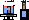
\includegraphics[width=0.65\textwidth]{bilder/versuchsaufbau_dulon_peptip.pdf}
  \caption{Schematische Darstellung eines Thermoelements}
  \label{fig:aufbau}
\end{figure}
Der Versuchsaufbau ist in Abbildung \ref{fig:aufbau} dargestellt.
Im Wesentlichen besteht der Versuch aus einem Kaloriemeter, einem Thermoelement,
Probemassen (Grafit, Zinn und Aluminium).
Zusätzlich werden noch ein Wasserbad mit Heizplatte und
ein mit Eiswasser gefüllten Dewargefäß benötigt.

\subsection{Versuchsdurchführung}
%\subsubsection{Kalibierung des Thermoelemtentes} Soll ich das auch machen ?

\subsubsection{Bestimmung der Wärmekapazität des Kalorimeters}
Um die Wärmekapazität des Kalorimeters zu bestimmen, werden 
zwei Wassermengen $m_x$ und $m_y$ mit der dazugehörigen Temperatur $T_x$ und $T_y$ 
im Kalorimeter vermischt. 
Die sich einstellende Mischtemperatur $T_M$ wird durch ein Thermoelement gemessen.
Dabei sei einer der beiden Kontaktstellen
in einem mit Eiswasser gefüllten Deware-Gefäß.
Mittels $T_M$ und \eqref{eq:zusammenhang_cgmg} kann dann auf die Wärmekapazität des 
Kaloriemeters geschlossen werden.

\subsubsection{Bestimmung der Wärmekapazität}
Zu Anfang des Versuches wird ein Dewargefäß mit Eiswasser gefüllt.
Eine Kontaktstelle des Thermoelements wird in das Eiswasser gegeben.
Es dient für weitere Temperaturmessung als Referenzpunkt.
Generell werden alle Temperaturmessungen mit einem Thermoelement ausgeführt.
Anschließend wird ein Probekörper in einem Wasserbad erhitzt.
Während dessen wird ein weiters Deware-Gefäßs mit $\SI{600}{\milli\liter}$ Wasser gefüllt.
In ihm soll die Messung der Mischtemperatur erfolgen.
Dazu wird der erhitzte Probekörper in das Wasser geben.
Bevor wird jedoch noch die Temperatur vom Probekörper und die des Wassers gemessen.
Nachdem der Probekörper im Deware-Gefäß platziert wurde, wird die Mischtemperatur des
Wassers gemessen. Der Vorgang wird für Grafit und Zinn jeweils drei Mal und für
Aluminium einmal wiederholt.

